\subsection{Summing}

Initially we take the circuit built in Figure \ref{fig:CD_Sum} and we then inputted signals into the summer to see how well the summed signals compared to the theoretical signals which we expected to get. We graph the inputted signals and the outputted data on the same graph, and then we numerically sum the data and compare the theoretical signal to the outputted data by taking a difference of the two values. This gives us our second graph shown on the right.

In Equation \ref{eqn:sum} it can be seen that the the Voltages are scaled by a factor, this factor was calculated by referencing Table \ref{tab:components} and noting that $R_1$ = $R_1$, $R_2$ = $R_2$ and $R_f$ = $R_3$. These gains are nearly 1 in both cases unity, and are included for completeness, but we saw that they were small enough to not noticeably change the shape of the data.

Here we will show multiple graphs, starting with sine waves at various frequencies:

\begin{figure}[h!]
\centering
\begin{subfigure}[t]{.475\textwidth}
  \centering
  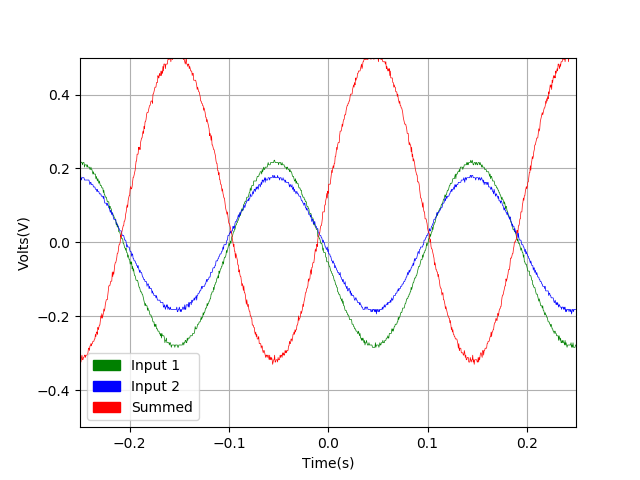
\includegraphics[width=0.95\textwidth, height=0.20\textheight]{figures/Summing/scope_1raw.png}
  \caption{The raw data from the oscilloscope. Inputs (V1, V2) and the Summed Signal (V0)}
 \label{fig:sum_1_og_data}
\end{subfigure}\hfill
\begin{subfigure}[t]{.475\textwidth}
  \centering
  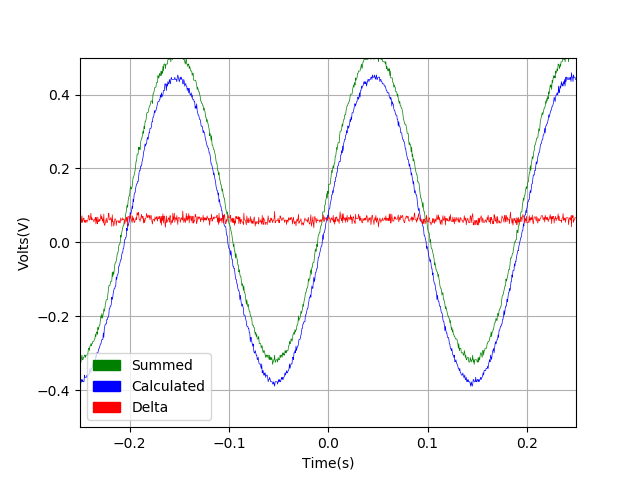
\includegraphics[width=0.95\textwidth, height=0.20\textheight]{figures/Summing/scope_1.png}
  \caption{The summed raw data (V), calculated signal -($v_1 + v_2$) \& difference between them (delta).}
\label{fig:sum_1_calc_data}
\end{subfigure}
\caption{Sine waves Summed with 0 phase difference, 5Hz signal}
\label{fig:sum_1}
\end{figure}
\begin{figure}[h!]
\centering
\begin{subfigure}[t]{.475\textwidth}
  \centering
  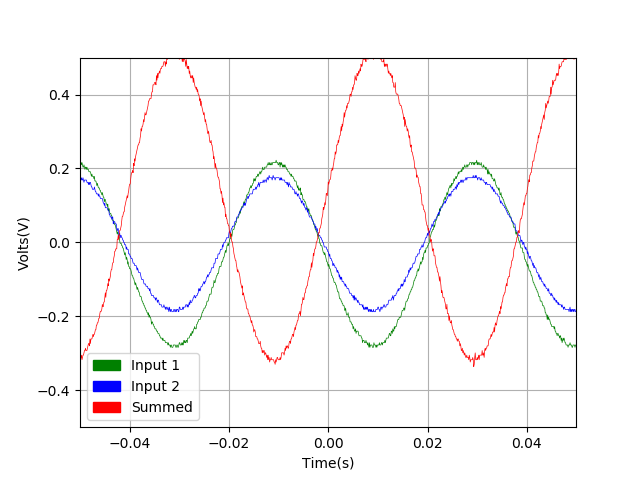
\includegraphics[width=0.95\textwidth, height=0.20\textheight]{figures/Summing/scope_2raw.png}
  \caption{The raw data from the oscilloscope. Inputs (V1, V2) and the Summed Signal (V0)}
 \label{fig:sum_2_og_data}
\end{subfigure}\hfill
\begin{subfigure}[t]{.475\textwidth}
  \centering
  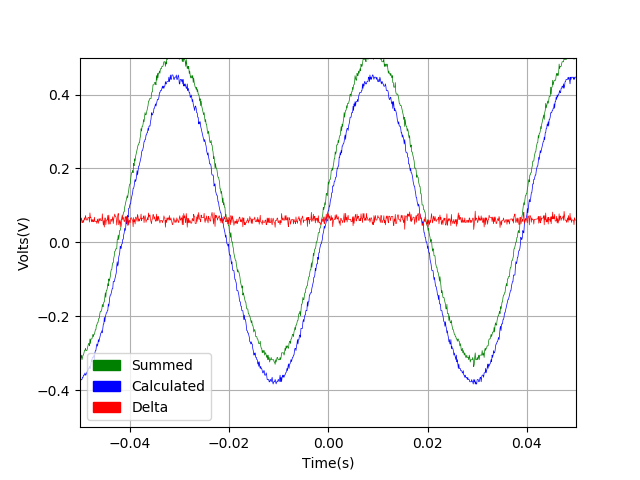
\includegraphics[width=0.95\textwidth, height=0.20\textheight]{figures/Summing/scope_2.png}
  \caption{The summed raw data (V), calculated signal -($v_1 + v_2$)\& difference between them (delta).}
\label{fig:sum_2_calc_data}
\end{subfigure}
\caption{Sine waves Summed with 0 phase difference, 25Hz signal}
\label{fig:sum_2}
\end{figure}

From Figures \ref{fig:sum_1} \& \ref{fig:sum_2} we can see that the difference between 25Hz and 5Hz signals show no clear sign of difference between the two, if there is any significant difference it is dominated by the noise of the signal. We do notice that there is a DC difference between the two signals, which is caused by the digital DC offset which was set by ourselves in the lab to differentiate the signals visually. However this does not explain all of the signal as these DC offsets lead to a 83.5mV difference from zero, but we see a consistent 61 $\pm 2$ mV signal found from the delta. This implies that there is a small DC element which is being added into the summed signal. 

%Precious comment before line width was decreased. Untrue now
%pattern emerge due to the Frequency of the data. We see that the low frequency data has a much ``cleaner'' signal, which means that the calculated summation is much closer to the real signal as compared to the 25 Hz signal. We can also see that the 10Hz signal (Figure \ref{fig:sum_0}) is in between the two. This can be thought of as expected as the op-amp has to ``react'' to the change in the signal, as it takes time for the signal to propagate through the op-amp and giving a slower signal will allow for it to keep up.
%\newline

We now take a look into phase differences, we focus first on the sine waves again as a test case:

\begin{figure}[h!]
\centering
\begin{subfigure}[t]{.475\textwidth}
  \centering
  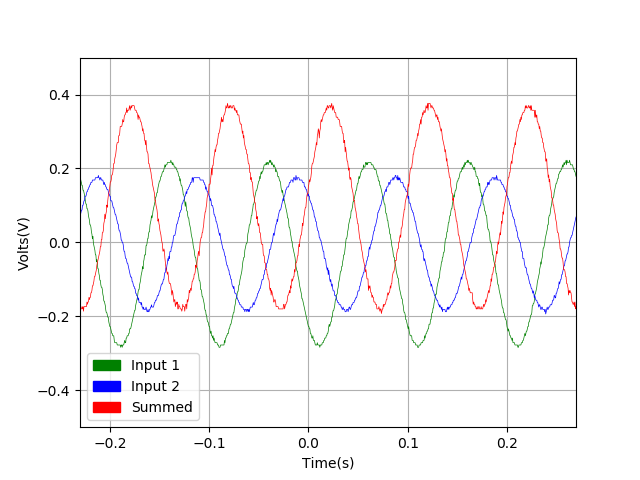
\includegraphics[width=0.95\textwidth, height=0.22\textheight]{figures/Summing/scope_3raw.png}
  \caption{The raw data from the oscilloscope. Inputs (V1, V2) and the Summed Signal (V0)}
 \label{fig:sum_3_og_data}
\end{subfigure}\hfill
\begin{subfigure}[t]{.475\textwidth}
  \centering
  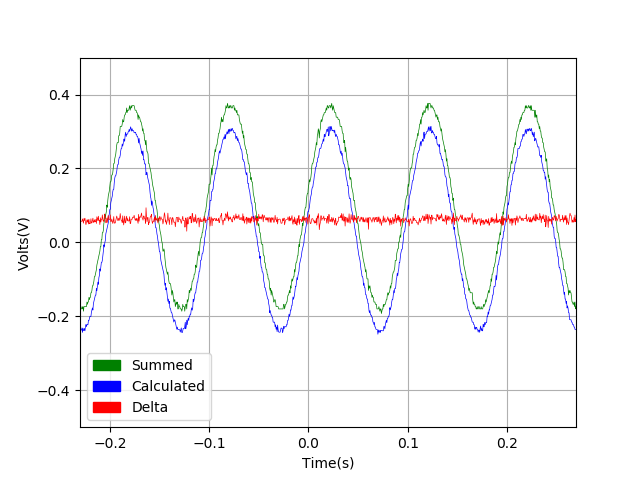
\includegraphics[width=0.95\textwidth, height=0.22\textheight]{figures/Summing/scope_3.png}
  \caption{The summed raw data (V), calculated signal -($v_1 + v_2$)\& difference between them (delta).}
\label{fig:sum_3_calc_data}
\end{subfigure}
\caption{Sine waves Summed with 90$^\circ$ phase difference, 10Hz signal}
\label{fig:sum_3}
\end{figure}

\begin{figure}[h!]
\centering
\begin{subfigure}[t]{.475\textwidth}
  \centering
  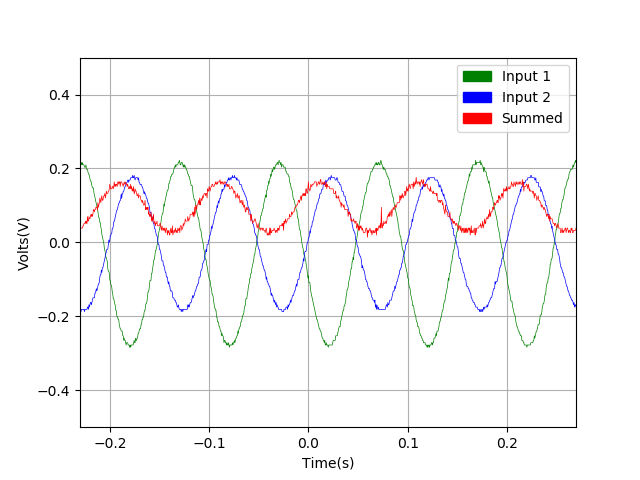
\includegraphics[width=0.95\textwidth, height=0.24\textheight]{figures/Summing/scope_5raw.png}
  \caption{The raw data from the oscilloscope. Inputs (V1, V2) and the Summed Signal (V0)}
 \label{fig:sum_5_og_data}
\end{subfigure}\hfill
\begin{subfigure}[t]{.475\textwidth}
  \centering
  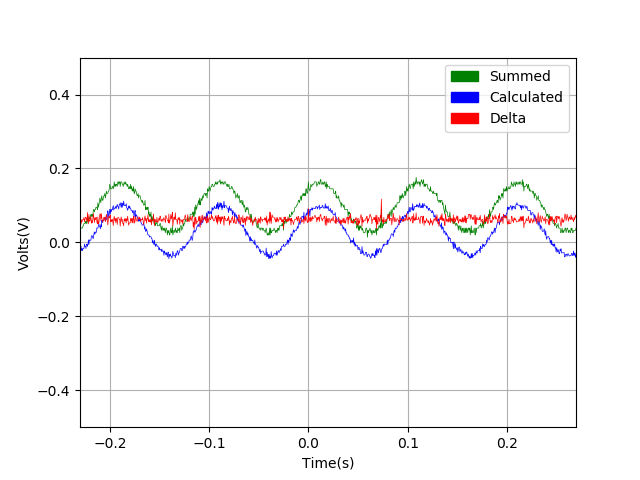
\includegraphics[width=0.95\textwidth, height=0.24\textheight]{figures/Summing/scope_5.png}
  \caption{The summed raw data (V), calculated signal -($v_1 + v_2$)\& difference between them (delta).}
\label{fig:sum_5_calc_data}
\end{subfigure}
\caption{Sine waves Summed with 170$^\circ$ phase difference, 10Hz signal}
\label{fig:sum_5}
\end{figure}

We see that the phase difference appears to make no visible difference to the amount of difference between the calculated and found signal. This is concluded by observing the difference in size and shape of the delta signal between Figures \ref{fig:sum_3} \& \ref{fig:sum_5}. However as a percentage of signal it is important to note that deconstructive interference lead to the case where the noise in the delta signal is significant compared to the signal (Figure \ref{fig:sum_9}). 
\newline

At this point we also note that many other combinations of signals were completed and are presented in Appendix \ref{append:sum}. These were also done with varying phase factors, but these simply followed the pattern of the points stated above. We show three examples here, the first two are shown in Figures \ref{fig:sum_7} \& \ref{fig:sum_11} shows that the addition of non-sine wave functions works similarly to summations seen of sine waves, even with odd phase differences.
\begin{figure}[h!]
\centering
\begin{subfigure}[t]{.475\textwidth}
  \centering
  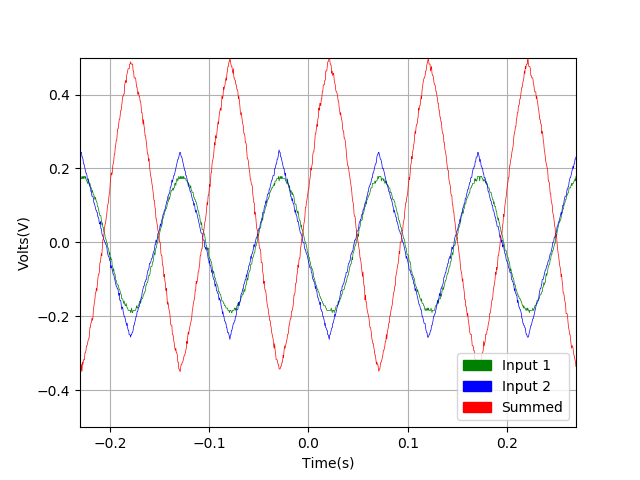
\includegraphics[width=0.95\textwidth, height=0.25\textheight]{figures/Summing/scope_7raw.png}
  \caption{The raw data from the oscilloscope. Inputs (V1, V2) and the Summed Signal (V0)}
 \label{fig:sum_7_og_data}
\end{subfigure}\hfill
\begin{subfigure}[t]{.475\textwidth}
  \centering
  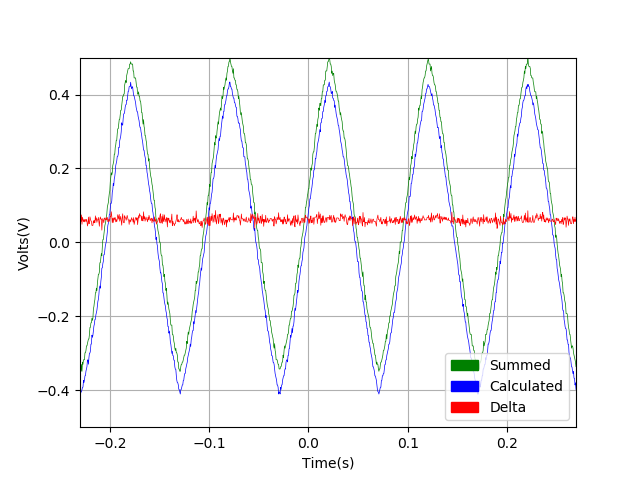
\includegraphics[width=0.95\textwidth, height=0.25\textheight]{figures/Summing/scope_7.png}
  \caption{The summed raw data (V), calculated signal -($v_1 + v_2$)\& difference between them (delta).}
\label{fig:sum_7_calc_data}
\end{subfigure}
\caption{Sine wave summed with a triangular wave, 10Hz signal}
\label{fig:sum_7}
\end{figure}

\begin{figure}[h!]
\centering
\begin{subfigure}[t]{.475\textwidth}
  \centering
  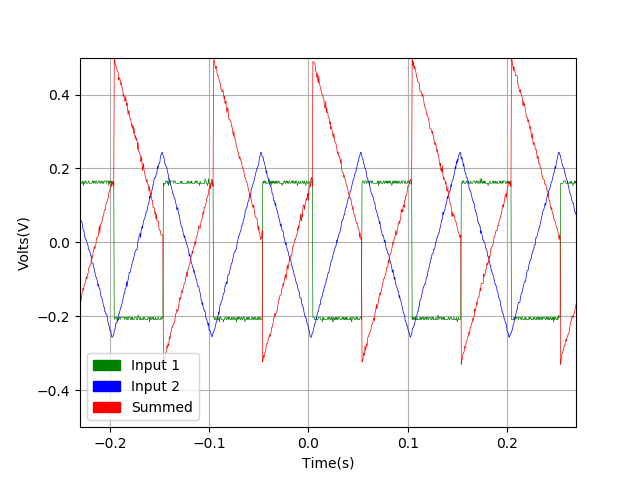
\includegraphics[width=0.95\textwidth, height=0.25\textheight]{figures/Summing/scope_11raw.png}
  %\caption{The raw data from the oscilloscope. Inputs (V1, V2) and the Summed Signal (V0)}
 \label{fig:sum_11_og_data}
\end{subfigure}\hfill
\begin{subfigure}[t]{.475\textwidth}
  \centering
  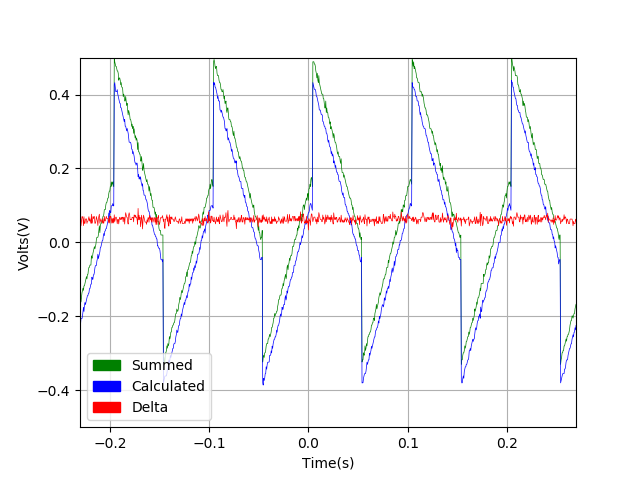
\includegraphics[width=0.95\textwidth, height=0.25\textheight]{figures/Summing/scope_11.png}
  %\caption{The summed raw data (V), calculated signal -($v_1 + v_2$)\& difference between them (delta).}
\label{fig:sum_11_calc_data}
\end{subfigure}
\caption{Square summed with a triangular, 10Hz signal, off phase by $\sim1/2$ wave}
\label{fig:sum_11}
\end{figure}

Then we take a look at Figure \ref{fig:sum_9}. This leads to our signal due to deconstructive interference, but the noise still dominates any significant issues that we are able to see in the data. The variance of each of the deltas is seen to be constant, leading us to conclude that the different setups did not cause significant differences in output.
\begin{figure}[h!]
\centering
\begin{subfigure}[t]{.475\textwidth}
  \centering
  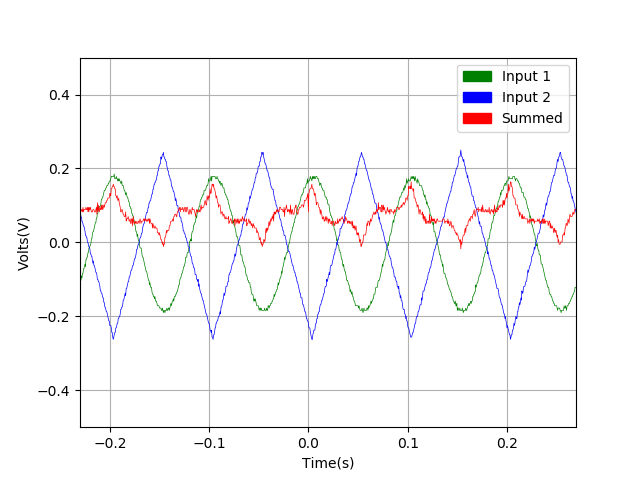
\includegraphics[width=0.95\textwidth, height=0.22\textheight]{figures/Summing/scope_9raw.png}
  \caption{The raw data from the oscilloscope. Inputs (V1, V2) and the Summed Signal (V0)}
 \label{fig:sum_9_og_data}
\end{subfigure}\hfill
\begin{subfigure}[t]{.475\textwidth}
  \centering
  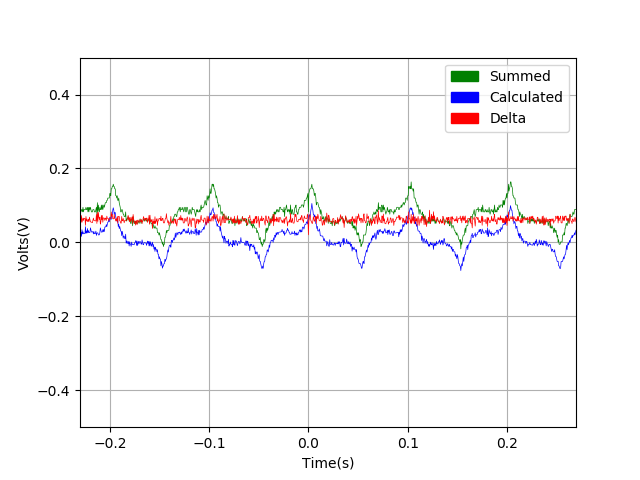
\includegraphics[width=0.95\textwidth, height=0.22\textheight]{figures/Summing/scope_9.png}
  \caption{The summed raw data (V), calculated signal -($v_1 + v_2$)\& difference between them (delta).}
\label{fig:sum_9_calc_data}
\end{subfigure}
\caption{Sine summed with a triangular, 10Hz signal, off by $\sim 1/2$ a wave}
\label{fig:sum_9}
\end{figure}
\subsection{Differentiation}

With the circuit built in Figure \ref{fig:CD_Diff} the inputted signals are taken, and the output is also taken then each of those signals are graphed against one another. Then a numerical differentiation is completed using custom Python software, which is simply calculated by finding the difference between the last point and current point. These are then appropriately scaled according to the known constant factors in Equation \ref{eqn:diff} based off of the reference values in Table \ref{tab:components}. This scaling factor is -$R_1 \times C_1$.

We first present the data found for the sine wave:

\begin{figure}[h!]
\centering
\begin{subfigure}[t]{.475\textwidth}
  \centering
  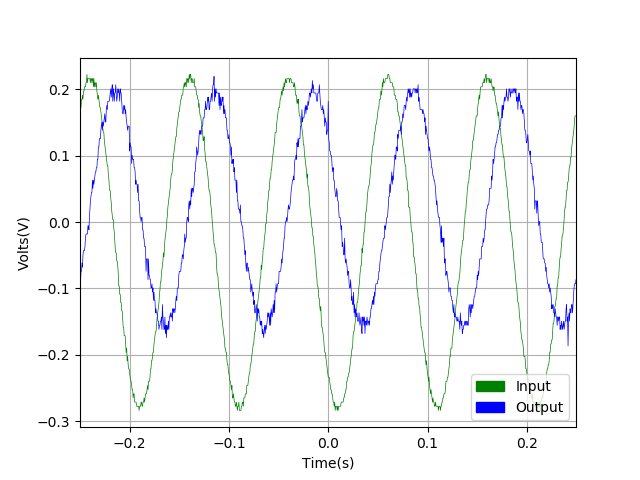
\includegraphics[width=0.95\textwidth, height=0.22\textheight]{figures/Differentiation/scope_19raw.png}
  \caption{The raw data from the oscilloscope. Inputted and Differentiated signal}
 \label{fig:diff_19_og_data}
\end{subfigure}\hfill
\begin{subfigure}[t]{.475\textwidth}
  \centering
  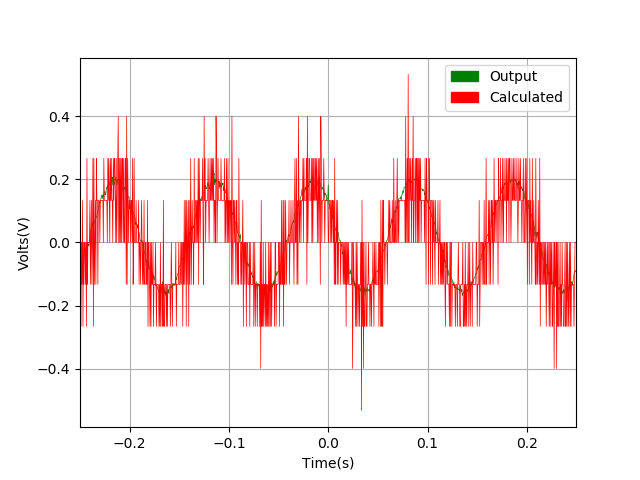
\includegraphics[width=0.95\textwidth, height=0.22\textheight]{figures/Differentiation/scope_19_calc_front.png}
  \caption{The summed raw data (V), and the numerically differentiated data.}
\label{fig:diff_no_filter}
\end{subfigure}
\caption{Differentiated sine wave with numerical differentiation compared to the analogue differentiation}
\label{fig:diff_sine}
\end{figure}

We see that in Figure \ref{fig:diff_19_og_data} we have a signal which looks to be differentiated, and we see that it creates a sine wave with a phase difference. This phase difference appears to be 90$^\circ$, which is consistent with how an inverted cos wave would appear, which is in fact what the differentiated signal should be, due to the negative scaling factor from the inverting op-amp. 

%The sine wave is expected to occur as we scale the data by a negative number, which means that the cosine which the sine wave differentiates into will appear to be flipped again, returning to be a sine wave. 

%However the phase difference is an unexpected, and we think that this is caused by a reaction time of the analogue circuitry, as the capacitor and op-amp will both take some time to function. The RC time constant is 10.64 ms with a negligible measurement error, by looking at the differences in peaks we see that their separation is also on the order of 12 $\pm 5$ ms. Measurements completed at different frequencies would help establish if this is the major reason as to why this phase difference exists. \newline

Figure \ref{fig:diff_no_filter} is striking, as we see that it is highly noisy, and if detail is paid to the values it can be seen that the points only lie on a ``quantized'' levels. These levels are likely due to the ADC which is built into the oscilloscope itself, meaning that the numerical differentiation will be limited by these levels as well.\newline

Here we present the results of filtering which will clean up our data:

\begin{figure}[h!]
\centering
\begin{subfigure}[t]{.475\textwidth}
  \centering
  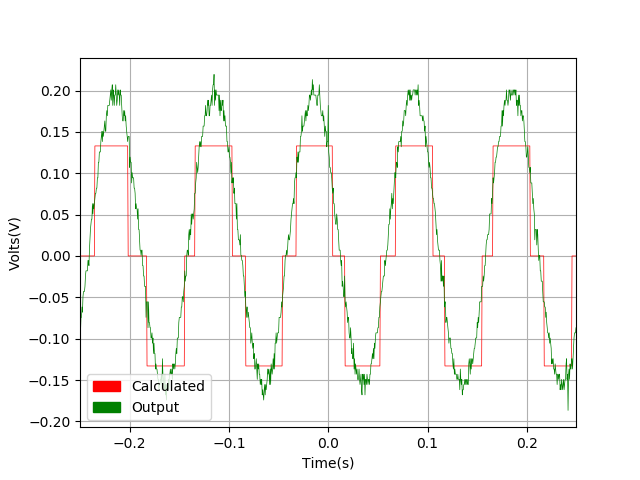
\includegraphics[width=0.95\textwidth, height=0.22\textheight]{figures/Differentiation/scope_19_calc_behind.png}
  \caption{The raw data output of the oscilloscope compared with the filtered numerical result.}
 \label{fig:diff_19}
\end{subfigure}\hfill
\begin{subfigure}[t]{.475\textwidth}
  \centering
  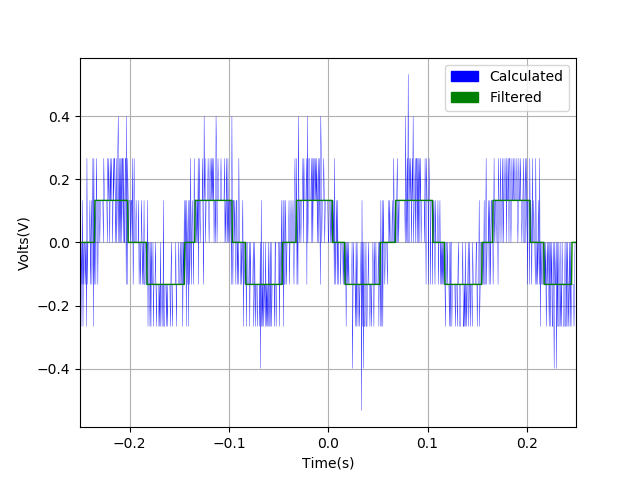
\includegraphics[width=0.95\textwidth, height=0.22\textheight]{figures/Differentiation/scope_19diff_filtered.png}
  \caption{The numerical differentiation compared with the filtered numerical result.}
\label{fig:diff_19_filter_compare}
\end{subfigure}
\caption{Filtering of the sine wave to show the numerical differentiation.}
\label{fig:diff_sine}
\end{figure}

Here we have shown the effect of filtering. This filtering is median filtering which simply takes the median value which is found in the window. Hence there is no interpolation, which means that we can clearly see the ``quantized'' levels created by the ADC. We can also see that it generally follows the trend of the expected graph. I will note that the median filter is of 41 points which relates to a 20.5 ms window, and the waves appear to be in phase, although it is difficult to establish as the filtering obscures the peaks. \newline

We will next look at differentiating the triangular wave in Figure \ref{fig:diff_triangular}. We see in this that the triangular wave differentiated appears to be a square wave, this is what we would expect. We see that the amplitude of the numerically differentiated signal is also below that of the actual signal which is not surprising due to the issues discussed earlier.

\begin{figure}[h!]
\centering
\begin{subfigure}[t]{.475\textwidth}
  \centering
  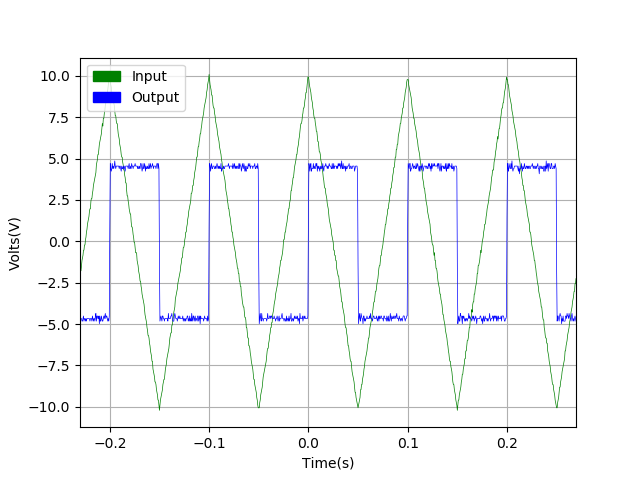
\includegraphics[width=0.95\textwidth, height=0.20\textheight]{figures/Differentiation/scope_15raw.png}
  \caption{The raw data input and output of the scope}
 \label{fig:diff_triangular_raw}
\end{subfigure}\hfill
\begin{subfigure}[t]{.475\textwidth}
  \centering
  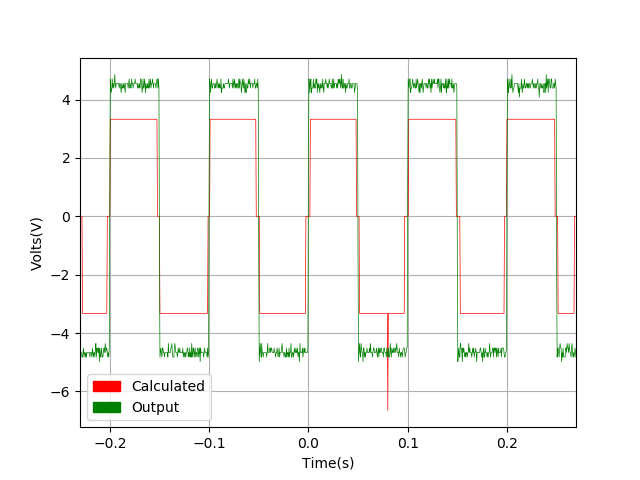
\includegraphics[width=0.95\textwidth, height=0.20\textheight]{figures/Differentiation/scope_15_calc_behind.png}
  \caption{The filtered numerical differentiation compared with the output signal.}
\label{fig:diff_triangular_filter}
\end{subfigure}
\caption{Differentiated triangular wave signal.}
\label{fig:diff_triangular}
\end{figure}

From visual analysis we are also able to pick up another detail of the analogue computer. For the triangular wave this is shown in the Figure \ref{fig:diff_triangular_analouge}. We are able to see the RC bounce which occurs because of the analogue circuitry overshooting equilibrium and then stabilizing down to it. We note that this occurs over about 1 ms, which is 10\% of the RC time constant which is 10.64 ms. \newline

\begin{figure}[h!]
\centering
\begin{subfigure}[t]{.475\textwidth}
  \centering
  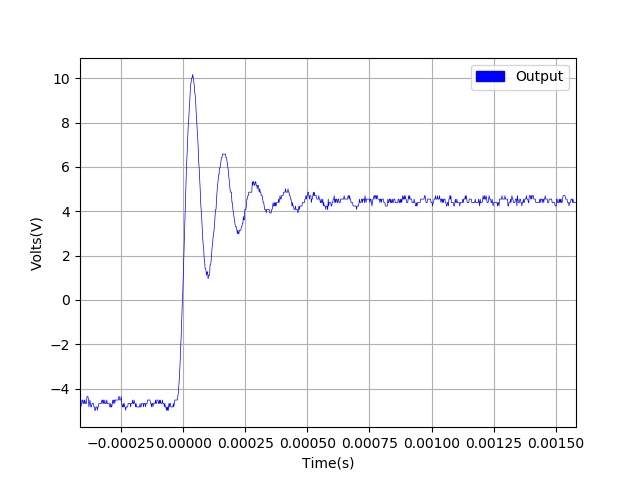
\includegraphics[width=0.95\textwidth, height=0.22\textheight]{figures/Differentiation/scope_16raw_out.png}
  \caption{The raw data output of the triangular wave differentiation, showing RC bounce.}
 \label{fig:diff_triangular_analouge}
\end{subfigure}\hfill
\begin{subfigure}[t]{.475\textwidth}
  \centering
  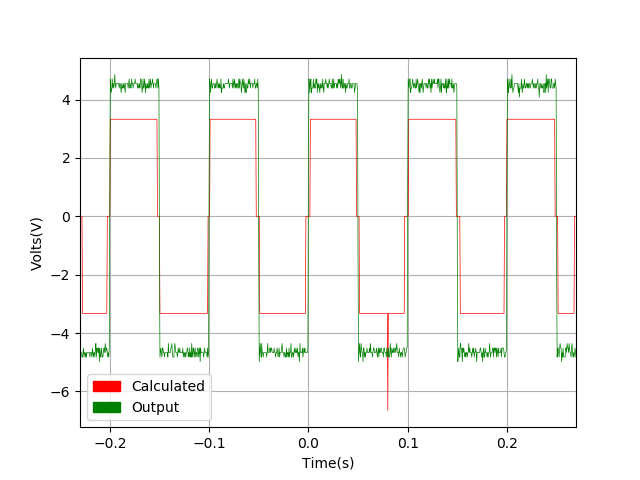
\includegraphics[width=0.95\textwidth, height=0.22\textheight]{figures/Differentiation/scope_15_calc_behind.png}
  \caption{The raw data output of the square wave differentiation compared to the calculated}
\label{fig:diff_square_analouge}
\end{subfigure}
\caption{Analogue effects seen in the circuitry.}
\label{fig:diff_analouge}
\end{figure}

We now take a look at the square wave input. We see that the square differentiated signal creates a large dirac delta peak, which is again as expected. We do not median filter this data as median filtering would remove the sharp peak. In the unfiltered data we see that the peak is bigger in the calculated data then it is in the real data. When looking at this effect at a higher resolution we see Figure \ref{fig:diff_square_analouge}. This is why we see the peak as lower and wider than the real delta peak. We see that this analogue effect of the capacitor discharging is causing this. \newline

\begin{figure}[h!]
\centering
\begin{subfigure}[t]{.475\textwidth}
  \centering
  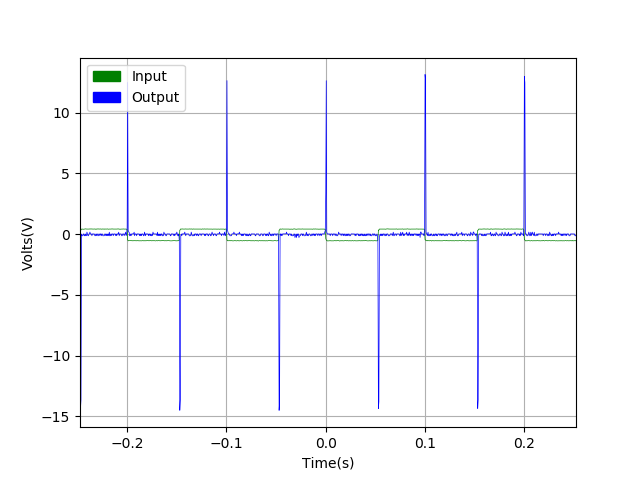
\includegraphics[width=0.95\textwidth, height=0.20\textheight]{figures/Differentiation/scope_17raw.png}
  \caption{The raw data input and output of the scope}
 \label{fig:diff_triangular_raw}
\end{subfigure}\hfill
\begin{subfigure}[t]{.475\textwidth}
  \centering
  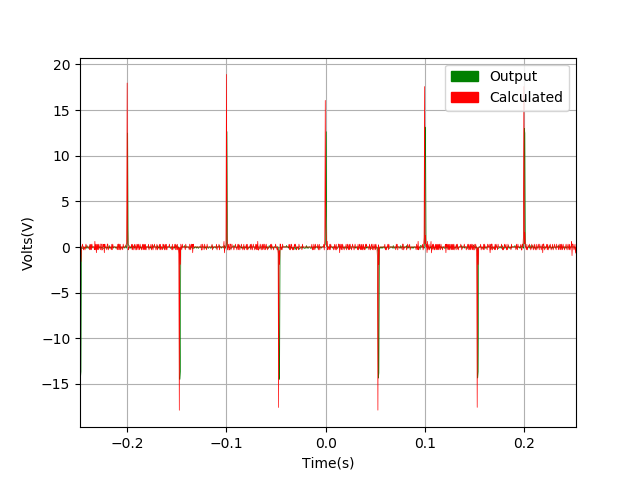
\includegraphics[width=0.95\textwidth, height=0.20\textheight]{figures/Differentiation/scope_17_calc_front.png}
  \caption{The numerical differentiation compared with the output signal.}
\label{fig:diff_triangular_unfilter}
\end{subfigure}
\caption{Differentiated square wave signal.}
\label{fig:diff_triangular}
\end{figure}

In the Appendix \ref{append:diff} we present the results of the DC coupling. We see in Figures \ref{fig:diff_DC} and \ref{fig:diff_AC} that we are unable to differentiate between the two situations. This is caused by the capacitor on the input of the differentiation circuit which means that the DC vs AC coupling will have no difference as the capacitor will remove any DC component to the signal anyways.

\subsection{Integration}
For this part of the lab we take the circuit built in Figure \ref{fig:CD_Int} and we then inputted signals into the integrator, to see that the signals were integrated. We then verified that the output signal was what we expected before we saved the data.

In Equation \ref{eqn:int} it can be seen that the the Voltages are scaled by a factor, this factor was calculated by referencing Table \ref{tab:components} and noting that $R_2$ = $R_2$ $C_3 = C_3$ and $C_b$ = $R_2$. 

Here we will show multiple graphs frequencies:

\begin{figure}[h!]
\centering
\begin{subfigure}[t]{.475\textwidth}
  \centering
  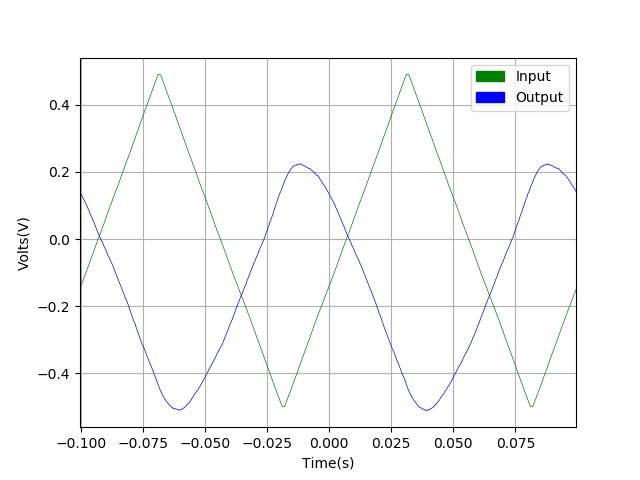
\includegraphics[width=0.95\textwidth, height=0.20\textheight]{figures/Intergration/scope_22raw.png}
  \caption{The raw data from the oscilloscope. Inputs (V1) and the Integrated Signal (V0)}
 \label{fig:int_1_og_data}
\end{subfigure}\hfill
\begin{subfigure}[t]{.475\textwidth}
  \centering
  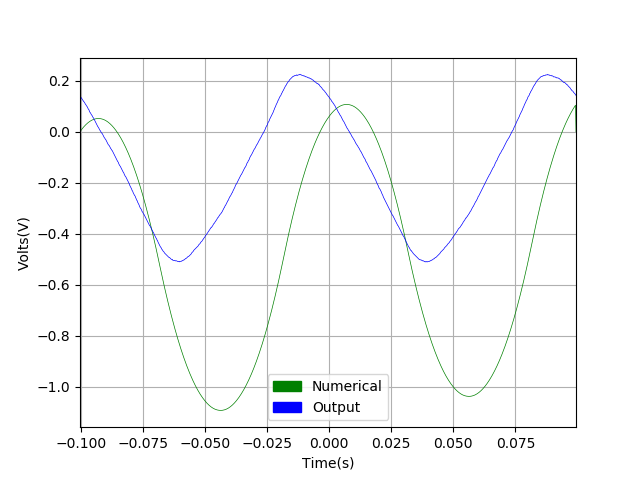
\includegraphics[width=0.95\textwidth, height=0.20\textheight]{figures/Intergration/scope_22.png}
  \caption{The integrated raw data (V), calculated signal -($\frac{-1}{RC}\int dV_i dt$).}
\label{fig:sum_1_calc_data}
\end{subfigure}
\caption{Triangular waves}
\label{fig:int_1}

\end{figure}
\begin{figure}[h!]
\centering
\begin{subfigure}[t]{.475\textwidth}
  \centering
  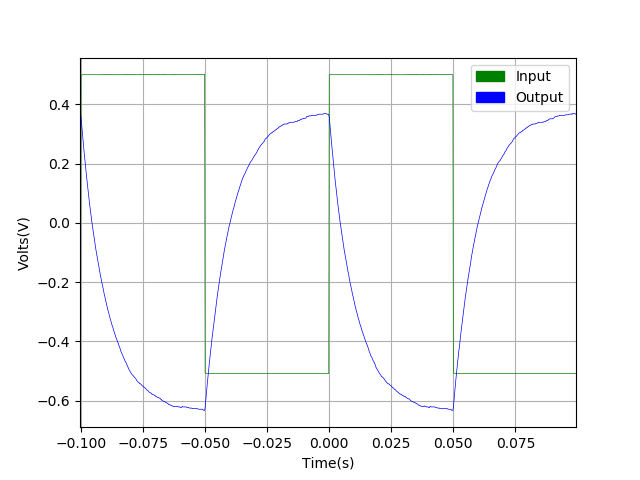
\includegraphics[width=0.95\textwidth, height=0.20\textheight]{figures/Intergration/scope_23raw.png}
  \caption{The raw data from the oscilloscope. Inputs (V1) and the Integrated Signal (V0)}
 \label{fig:int_2_og_data}
\end{subfigure}\hfill
\begin{subfigure}[t]{.475\textwidth}
  \centering
  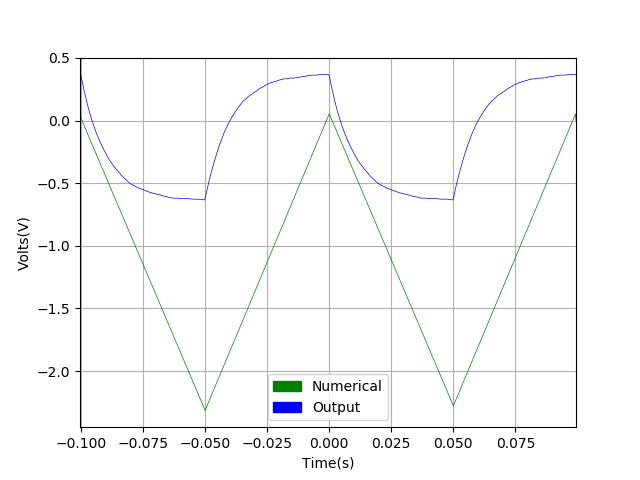
\includegraphics[width=0.95\textwidth, height=0.20\textheight]{figures/Intergration/scope_23.png}
  \caption{The integrated raw data (V), calculated signal -($\frac{-1}{RC}\int dV_i dt$).}
\label{fig:int_2_calc_data}
\end{subfigure}
\caption{Square Waves}
\label{fig:sum_2}
\end{figure}

Here we see that the calculated integrated wave and the raw output that was taken from the oscilloscope do not match very well, though the standard shape of each is kept. Th reason for this discrepancy may be because of the slew rate. The slew rate in an op-amp is the rate in change in the output voltage that is a direct result of the change in the step of the input voltage. This would lead to the distortion in the plots that we see. 

\begin{figure}[h!]
\centering
\begin{subfigure}[t]{.475\textwidth}
  \centering
  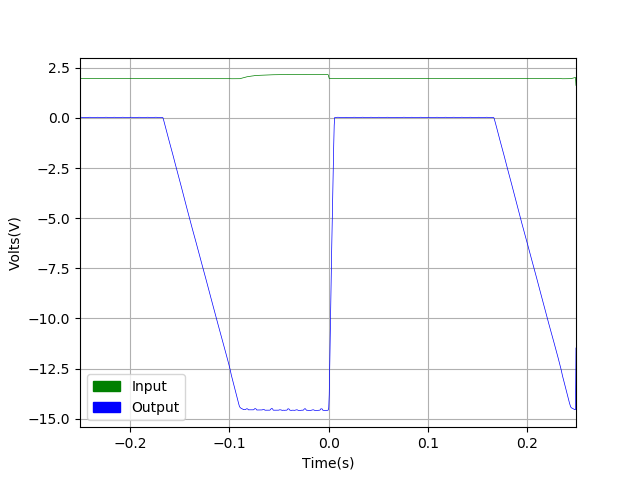
\includegraphics[width=0.95\textwidth, height=0.20\textheight]{figures/Intergration/scope_24raw.png}
  \caption{The raw data from the oscilloscope. The input is constant and the Integrated Signal (V0)}
 \label{fig:int_2_og_data}
\end{subfigure}\hfill
\begin{subfigure}[t]{.475\textwidth}
  \centering
  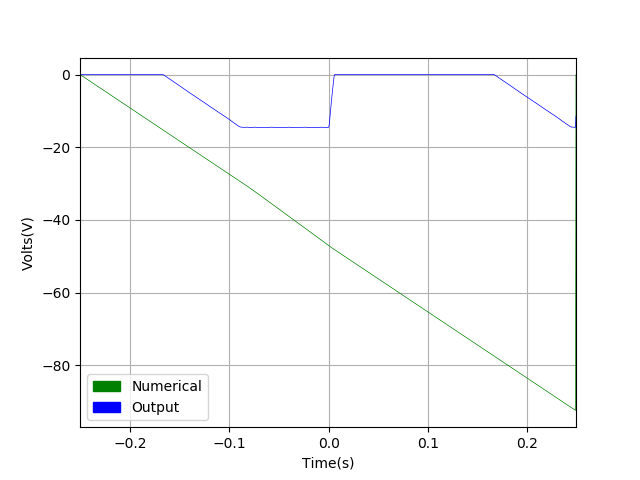
\includegraphics[width=0.95\textwidth, height=0.20\textheight]{figures/Intergration/scope_24.png}
  \caption{The integrated raw data (V), calculated signal -($\frac{-1}{RC}\int dV_i dt$).}
\label{fig:int_2_calc_data}
\end{subfigure}
\caption{A constant DC voltage was sent with the switch being controlled by a clock}
\label{fig:sum_2}
\end{figure}

\begin{figure}[h!]
\centering
\begin{subfigure}[t]{.475\textwidth}
  \centering
  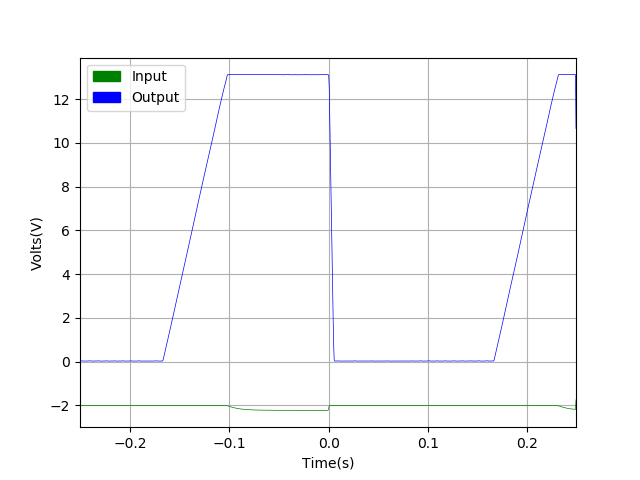
\includegraphics[width=0.95\textwidth, height=0.20\textheight]{figures/Intergration/scope_25raw.png}
  \caption{The raw data from the oscilloscope. The input is constant and the Integrated Signal (V0)}
 \label{fig:int_2_og_data}
\end{subfigure}\hfill
\begin{subfigure}[t]{.475\textwidth}
  \centering
  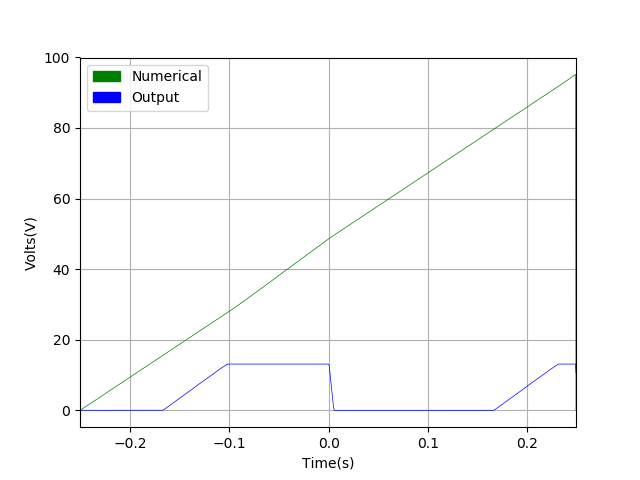
\includegraphics[width=0.95\textwidth, height=0.20\textheight]{figures/Intergration/scope_25.png}
  \caption{The integrated raw data (V), calculated signal -($\frac{-1}{RC}\int dV_i dt$).}
\label{fig:int_2_calc_data}
\end{subfigure}
\caption{A constant DC voltage was sent with the switch being controlled by a clock}
\label{fig:sum_2}
\end{figure}

The next part of this section we had to apply a DC voltage to the circuit to observe the voltage ramp at the output. We used a clock pulse in this to reset the voltage in place of the switch, that is why when you look at the output data you see that it comes in pulses. What we are looking for is the ramp that occurs before the new pulse. This is compared to the calculated ramp that we have, looking at the two graphs we see that the rate at which the two increase is very similar. 

In the two plots above we see a positive and negative constant input. We see from he graph that when you flip the input voltage from positive to negative. Our Oscilloscope was DC coupled which means that which means the it allowed for both the AC and DC current to pass through. This means that there is no extra capacitor that filters the DC current. 

\newpage

\subsection{Exponential} \label{sec:Exp}

We now setup the circuit as it is seen in Figure \ref{fig:CD_Exp}. This circuit will provide an exponential decay in the inputted signal as the signal is slowly reduced over time by the pentameter's resistor. We initially note that the solution will be of the form of $V_{out} = V_{in} = -RC \fran{d}{dt}V_{out}$ therefore the solution to the Voltage will be: $V = V_o e^{-1/RC}$. \newline

Therefore we graph the expected solution alongside the found signal, taking probes at before and after the op-amp. We show this here:

\begin{figure}[h!]
\centering
\begin{subfigure}[t]{.475\textwidth}
  \centering
  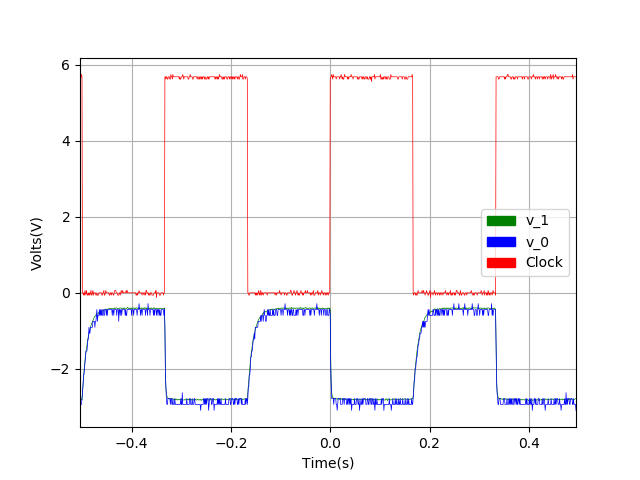
\includegraphics[width=0.95\textwidth, height=0.25\textheight]{figures/Exponential/scope_26raw.png}
  \caption{The raw data from the oscilloscope showing the signal before and after the op-amp.}
 \label{fig:Exp_0_raw}
\end{subfigure}\hfill
\begin{subfigure}[t]{.475\textwidth}
  \centering
  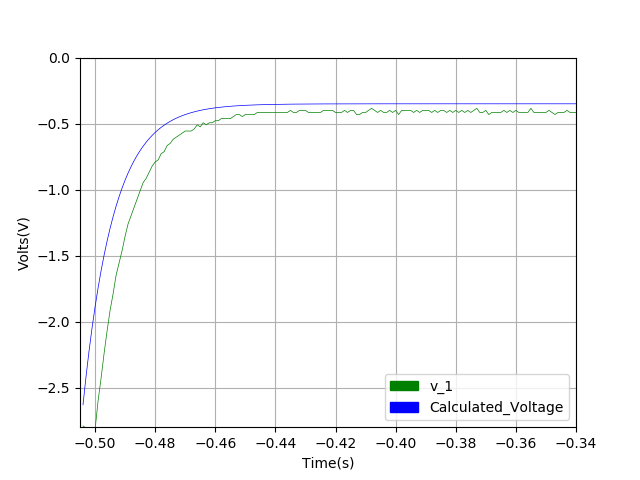
\includegraphics[width=0.95\textwidth, height=0.25\textheight]{figures/Exponential/scope_26_calc.png}
  \caption{The exponential graph along with our calculated signal.}
\label{fig:Exp_0_calc}
\end{subfigure}
\caption{The exponential solution of our circuit along with our expected signal.}
\label{fig:Exp_0}
\end{figure}

We see here that in Figure \ref{fig:Exp_0_calc} we have a very similar signal between our calculated and derived signal, however our solution is vertically and horizontally shifted. The horizontal shift is necessary as we start our exponential signal at the start point where the clock allows for the circuit to begin the exponential decay. However the vertical shift has less basis, we believe that the circuit should decay to 0 V, but instead we see that the voltage stays at -0.35 Volts. This deviation from theory is odd, and cannot be explained by digital shifts. It is also possible that the oscilloscope and the rest of the analogue circuitboard are at different grounds, but we see that the clock signal is properly set to zero therefore it is unlikely that the op-amp is referencing an incorrect ground. \newline

Moving on from this circuit we note that a solution of the form of $V = -(1 - \beta) \; e^{\frac{-(1 - \beta)}{RC}}$ where $\beta = \frac{R_pot}{R_o}$ where $R_o$ is the maximal resistance of the resistor. This presents us with solutions for our graph with progress as:

\begin{figure}[h!]
\centering
\begin{subfigure}[t]{.475\textwidth}
  \centering
  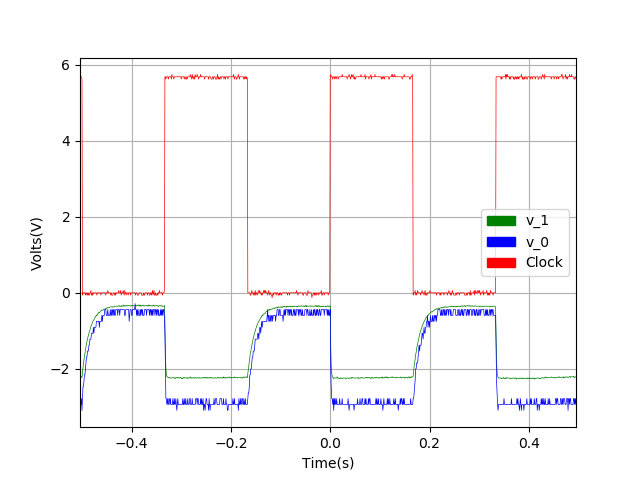
\includegraphics[width=0.95\textwidth, height=0.22\textheight]{figures/Exponential/scope_27raw.png}
  \caption{The raw data from the oscilloscope showing the signal before and after the op-amp.}
 \label{fig:Exp_2_raw}
\end{subfigure}\hfill
\begin{subfigure}[t]{.475\textwidth}
  \centering
  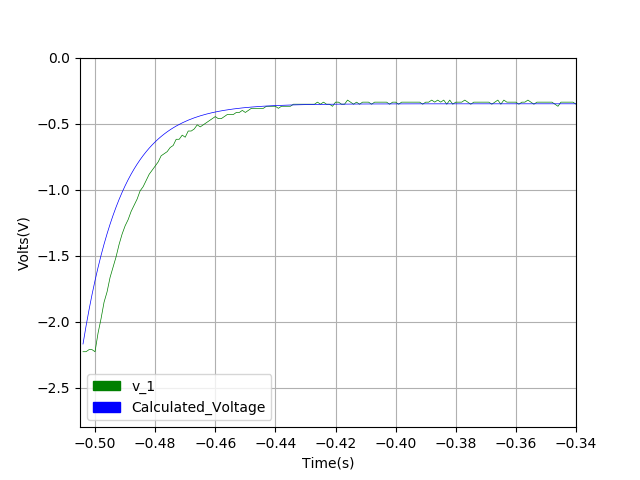
\includegraphics[width=0.95\textwidth, height=0.22\textheight]{figures/Exponential/scope_27_calc.png}
  \caption{The exponential graph along with our calculated signal.}
\label{fig:Exp_2_calc}
\end{subfigure}
\caption{The exponential solution of our circuit along with our expected signal for $\beta = 0.20$.}
\label{fig:Exp_2}
\end{figure}

\begin{figure}[h!]
\centering
\begin{subfigure}[t]{.475\textwidth}
  \centering
  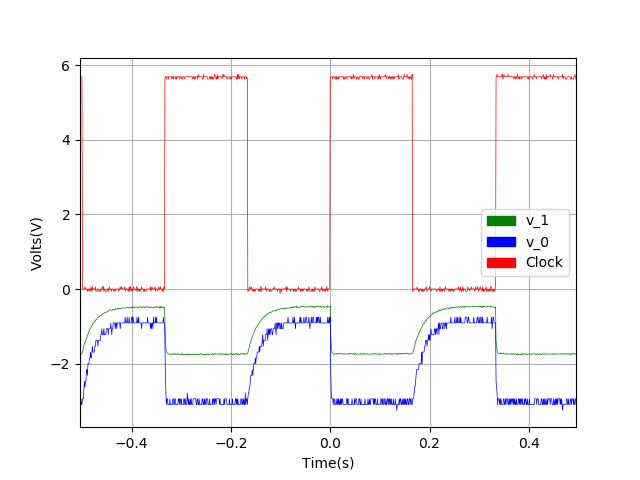
\includegraphics[width=0.95\textwidth, height=0.22\textheight]{figures/Exponential/scope_28raw.png}
  \caption{The raw data from the oscilloscope showing the signal before and after the op-amp.}
 \label{fig:Exp_4_raw}
\end{subfigure}\hfill
\begin{subfigure}[t]{.475\textwidth}
  \centering
  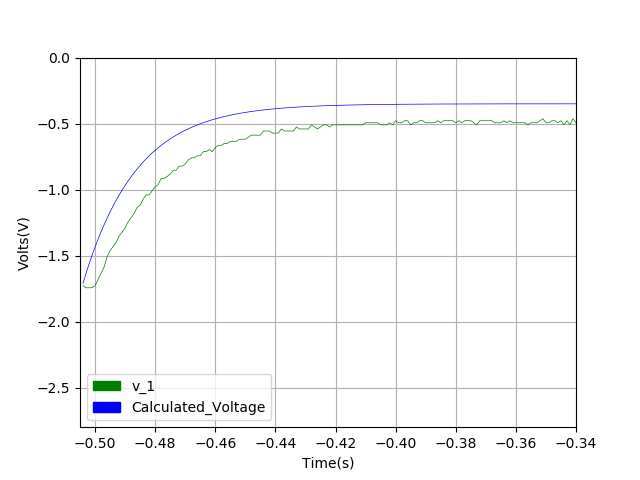
\includegraphics[width=0.95\textwidth, height=0.22\textheight]{figures/Exponential/scope_28_calc.png}
  \caption{The exponential graph along with our calculated signal.}
\label{fig:Exp_4_calc}
\end{subfigure}
\caption{The exponential solution of our circuit along with our expected signal for $\beta = 0.40$.}
\label{fig:Exp_4}
\end{figure}

\begin{figure}[h!]
\centering
\begin{subfigure}[t]{.475\textwidth}
  \centering
  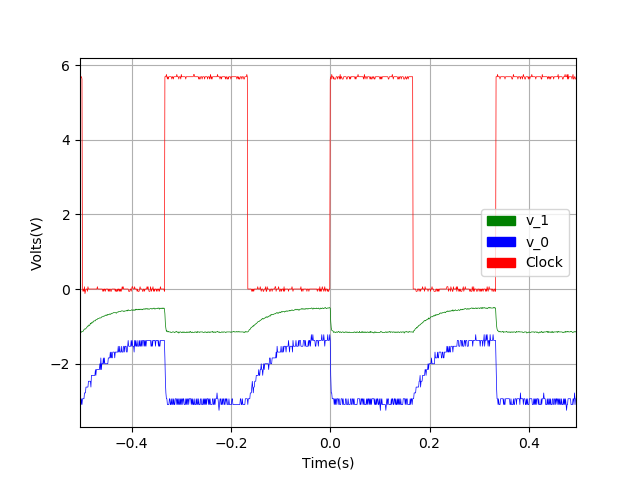
\includegraphics[width=0.95\textwidth, height=0.22\textheight]{figures/Exponential/scope_29raw.png}
  \caption{The raw data from the oscilloscope showing the signal before and after the op-amp.}
 \label{fig:Exp_6_raw}
\end{subfigure}\hfill
\begin{subfigure}[t]{.475\textwidth}
  \centering
  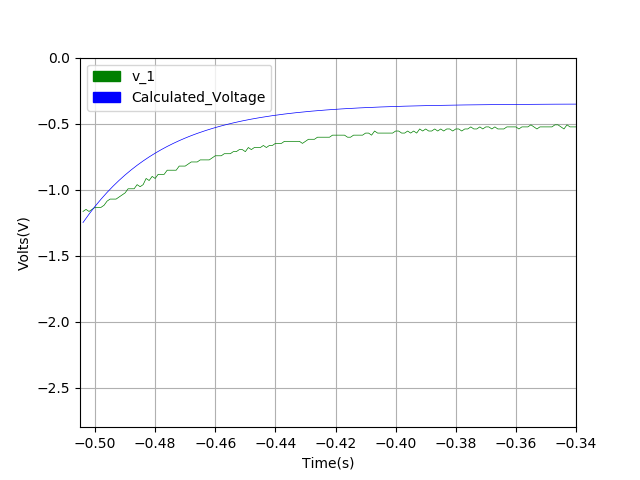
\includegraphics[width=0.95\textwidth, height=0.22\textheight]{figures/Exponential/scope_29_calc.png}
  \caption{The exponential graph along with our calculated signal.}
\label{fig:Exp_6_calc}
\end{subfigure}
\caption{The exponential solution of our circuit along with our expected signal for $\beta = 0.60$.}
\label{fig:Exp_6}
\end{figure}

We then present our solution and we can see that the correlation between our guessed solution and the experimentally found solution is strong. We see that the solutions for the lower ranged $\beta$ (0.20-0.60, as presented in Figure \ref{fig:Exp_2} to \ref{fig:Exp_6})) correlate well.

\begin{figure}[h!]
\centering
\begin{subfigure}[t]{.475\textwidth}
  \centering
  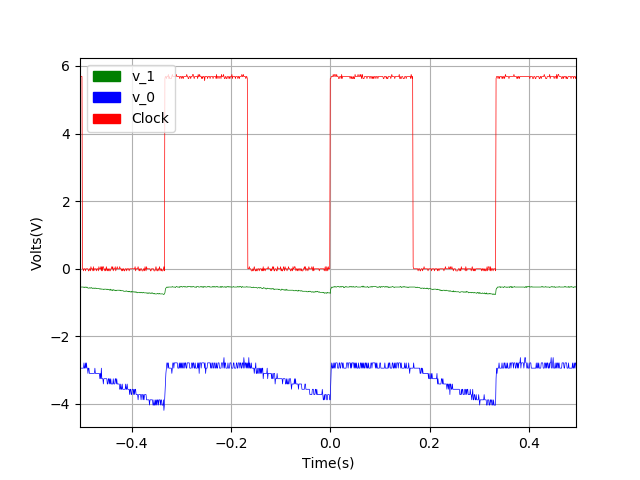
\includegraphics[width=0.95\textwidth, height=0.22\textheight]{figures/Exponential/scope_30raw.png}
  \caption{The raw data from the oscilloscope showing the signal before and after the op-amp.}
 \label{fig:Exp_8_raw}
\end{subfigure}\hfill
\begin{subfigure}[t]{.475\textwidth}
  \centering
  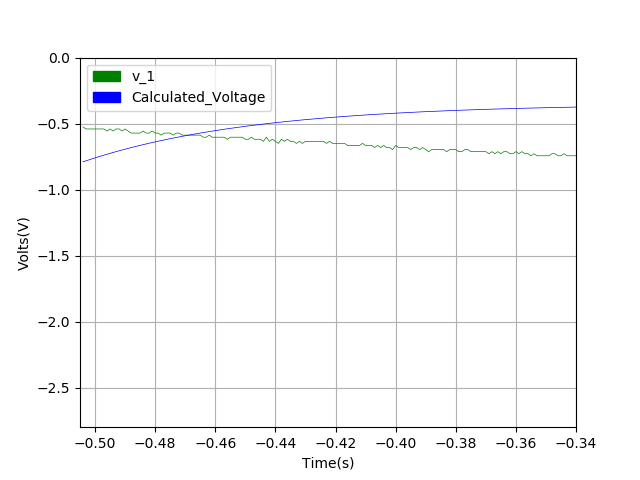
\includegraphics[width=0.95\textwidth, height=0.22\textheight]{figures/Exponential/scope_30_calc.png}
  \caption{The exponential graph along with our calculated signal.}
\label{fig:Exp_8_calc}
\end{subfigure}
\caption{The exponential solution of our circuit along with our expected signal for $\beta = 0.80$.}
\label{fig:Exp_8}
\end{figure}

\begin{figure}[h!]
\centering
\begin{subfigure}[t]{.475\textwidth}
  \centering
  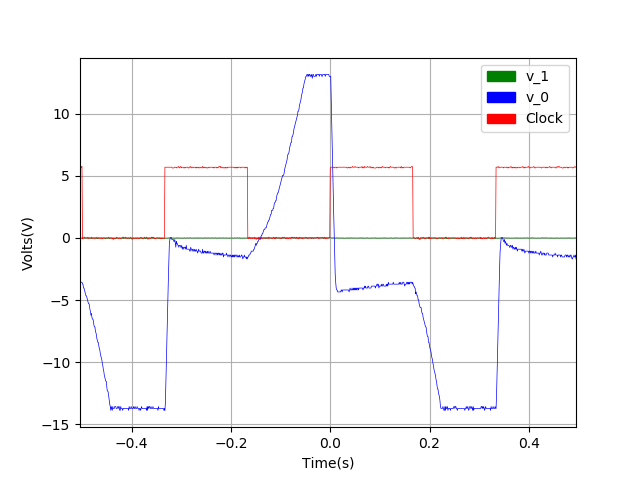
\includegraphics[width=0.95\textwidth, height=0.22\textheight]{figures/Exponential/scope_31raw.png}
  \caption{The raw data from the oscilloscope showing the signal before and after the op-amp.}
 \label{fig:Exp_10_raw}
\end{subfigure}\hfill
\begin{subfigure}[t]{.475\textwidth}
  \centering
  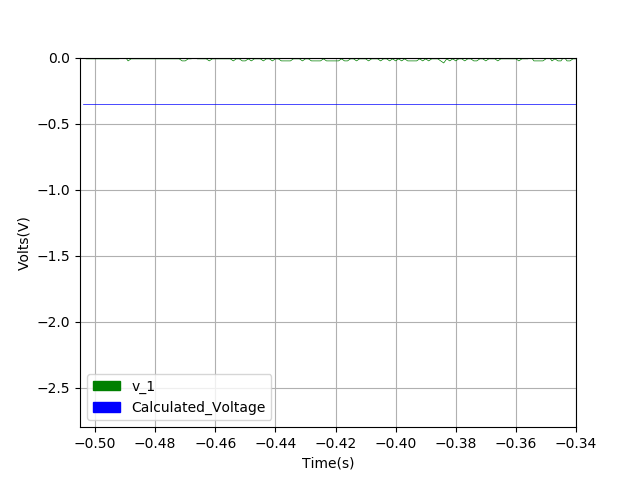
\includegraphics[width=0.95\textwidth, height=0.22\textheight]{figures/Exponential/scope_31_calc.png}
  \caption{The exponential graph along with our calculated signal.}
\label{fig:Exp_10_calc}
\end{subfigure}
\caption{The exponential solution of our circuit along with our expected signal for $\beta = 1.00$.}
\label{fig:Exp_10}
\end{figure}

However when we take a look at Figures \ref{fig:Exp_8} and \ref{fig:Exp_10} we see that the theory does not fare as well, however this is not unexpected as we are allowing very little of the original signal to be fed back into the input of the circuit again. This means that the signal is very low and the effect of ground noise and other imperfections in the op-amp and overall circuitry will become significant to the overall operating of the signal. To confirm this we see that the behaviour of the signals is relatively preserved in our limiting case (no feedback) of Figure \ref{fig:Exp_10_calc}, even though the very low signal case Figure \ref{fig:Exp_8_calc} has a different slope than is predicted by exponential decay.\newline

We also note that the signal which is being picked up as $v_0$ in Figure \ref{fig:Exp_10_raw} is unexpected, but it is not surprising that in the limiting case of a signal that there may be odd signal behaviour in the amplified integrated signal. However this behaviour is not explainable by us, but seems to be related to the capacitor based off of the signal's curvature, also it looks to be hitting the op-amp's rail voltages.

\clearpage
\subsection{Damped Harmonic Motion} \label{sec:DHO}

For this part of the lab we essentially combined all of the previous circuits, to make a circuit that has the solutions to damped harmonic motion, that as the equation $\ddot{V} + \frac{b}{m}\dot{V}+\frac{k}{m}V = 0$ At specific parts of the circuit we would measure the voltage and the plots below show our results. Those points we marked as $a,b,c,d$, where there
respective values were $\frac{d^2V}{dt^2}, \frac{-\frac{dV}{dt}}{RC}, \frac{V}{(RC)^2}, \frac{-V}{(RC)^2}$. The plots below detail the results that we found.

\begin{figure}[h!]
\centering
\begin{subfigure}[t]{.475\textwidth}
  \centering
  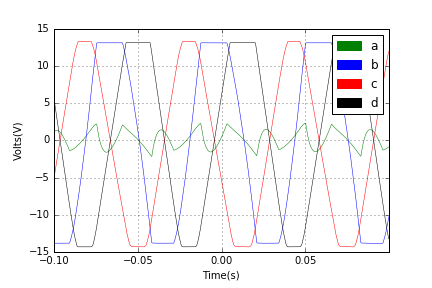
\includegraphics[width=0.95\textwidth, height=0.25\textheight]{figures/DHO/scope_35raw.png}
  \caption{The raw data from the oscilloscope, where a,b,c,d are all the voltages that are read}
 \label{fig:sum_7_og_data}
\end{subfigure}\hfill
\begin{subfigure}[t]{.475\textwidth}
  \centering
  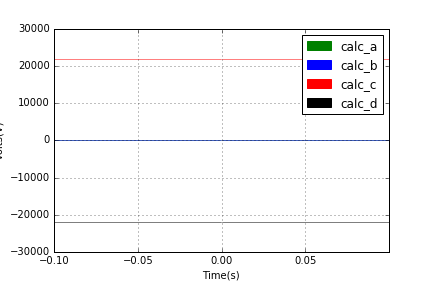
\includegraphics[width=0.95\textwidth, height=0.25\textheight]{figures/DHO/scope_35calc.png}
  \caption{The calculated values of a,b,c,d based on the corresponding equations}
\label{fig:sum_7_calc_data}
\end{subfigure}
\caption{For this on $R = 0.00k\Omega$}
\label{fig:sum_7}
\end{figure}

\begin{figure}[h!]
\centering
\begin{subfigure}[t]{.475\textwidth}
  \centering
  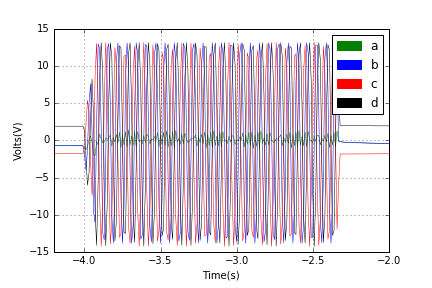
\includegraphics[width=0.95\textwidth, height=0.25\textheight]{figures/DHO/scope_36raw.png}
  \caption{The raw data from the oscilloscope, where a,b,c,d are all the voltages that are read}
 \label{fig:sum_7_og_data}
\end{subfigure}\hfill
\begin{subfigure}[t]{.475\textwidth}
  \centering
  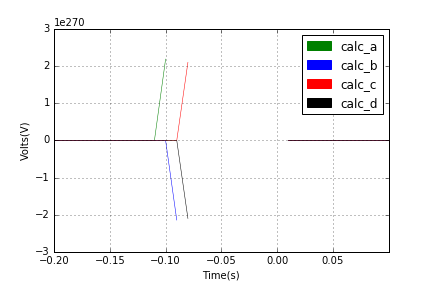
\includegraphics[width=0.95\textwidth, height=0.25\textheight]{figures/DHO/scope_36calc.png}
  \caption{The calculated values of a,b,c,d based on the corresponding equations}
\label{fig:sum_7_calc_data}
\end{subfigure}
\caption{For this on $R = 9.91k\Omega$}
\label{fig:sum_7}
\end{figure}

\begin{figure}[h!]
\centering
\begin{subfigure}[t]{.475\textwidth}
  \centering
  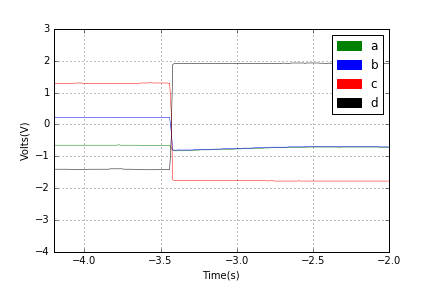
\includegraphics[width=0.95\textwidth, height=0.25\textheight]{figures/DHO/scope_37raw.png}
  \caption{The raw data from the oscilloscope, where a,b,c,d are all the voltages that are read}
 \label{fig:sum_7_og_data}
\end{subfigure}\hfill
\begin{subfigure}[t]{.475\textwidth}
  \centering
  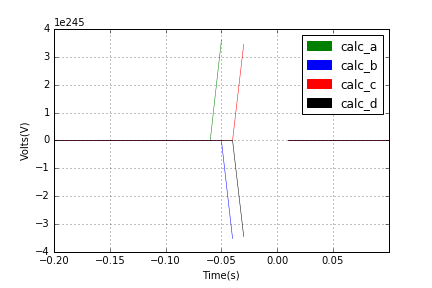
\includegraphics[width=0.95\textwidth, height=0.25\textheight]{figures/DHO/scope_37calc.png}
  \caption{The calculated values of a,b,c,d based on the corresponding equations}
\label{fig:sum_7_calc_data}
\end{subfigure}
\caption{For this on $R = 3.37k\Omega$}
\label{fig:sum_7}
\end{figure}
 It is evident from the graphs that the measured values do not match what we expect for a damp harmonic system. While completing the lab we looked at what could have caused this. The first thing that we looked at was to ensure that the circuit was properly built, which was the case. We then checked that each resistor and capacitor was of a correct value, that was not the cause, we kept investigating looking at the wires, the clock and were unable to determine the exact cause of the results that we obtained.
\clearpage

\subsection{Forced Damped Harmonic Motion} \label{sec:FDHO}

We can now add a signal generator which mean that the damped harmonic oscillator will reach a steady state. Therefore we have taken a ramp of the frequencies, and attempted to find the steady state amplitude for each. However due to issues with the Damped harmonic oscillator, we are unable to easily identify the exact section of steady state. We define the steady state to be reached at the middle of the graph (4-6 seconds) as before this we do not reach steady state in some of the graphs. This is seen best in Figure \ref{fig:FDHO_12Hz}. Also we see the damped harmonic oscillator fails after a certain point in Figure \ref{fig:FDHO_18Hz}, hence we attempt to capture the wave before this. 

\begin{figure}[h!]
\centering
\begin{subfigure}[t]{.475\textwidth}
  \centering
  \includegraphics[width=0.95\textwidth, height=0.20\textheight]{figures/FDHO/scope_39raw.png}
  \caption{The raw data from the oscilloscope showing a,b,c,d as in Section \ref{sec:DHO}.}
 \label{fig:FDHO_10Hz_raw}
\end{subfigure}\hfill
\begin{subfigure}[t]{.475\textwidth}
  \centering
  \includegraphics[width=0.95\textwidth, height=0.20\textheight]{figures/FDHO/scope_39v_2.png}
  \caption{The b output from the oscilloscope used to calculate the amplitude.}
\label{fig:FDHO_10Hz_b}
\end{subfigure}
\caption{The forced damped harmonic signal seen at 10Hz.}
\label{fig:FDHO_10Hz}
\end{figure}

\begin{figure}[h!]
\centering
\begin{subfigure}[t]{.475\textwidth}
  \centering
  \includegraphics[width=0.95\textwidth, height=0.20\textheight]{figures/FDHO/scope_40raw.png}
  \caption{The raw data from the oscilloscope showing a,b,c,d as in Section \ref{sec:DHO}.}
 \label{fig:FDHO_12Hz_raw}
\end{subfigure}\hfill
\begin{subfigure}[t]{.475\textwidth}
  \centering
  \includegraphics[width=0.95\textwidth, height=0.20\textheight]{figures/FDHO/scope_40v_2.png}
  \caption{The b output from the oscilloscope used to calculate the amplitude.}
\label{fig:FDHO_12Hz_b}
\end{subfigure}
\caption{The forced damped harmonic signal seen at 12Hz.}
\label{fig:FDHO_12Hz}
\end{figure}

\begin{figure}[h!]
\centering
\begin{subfigure}[t]{.475\textwidth}
  \centering
  \includegraphics[width=0.95\textwidth, height=0.20\textheight]{figures/FDHO/scope_43raw.png}
  \caption{The raw data from the oscilloscope showing a,b,c,d as in Section \ref{sec:DHO}.}
 \label{fig:FDHO_18Hz_raw}
\end{subfigure}\hfill
\begin{subfigure}[t]{.475\textwidth}
  \centering
  \includegraphics[width=0.95\textwidth, height=0.20\textheight]{figures/FDHO/scope_43v_2.png}
  \caption{The b output from the oscilloscope used to calculate the amplitude.}
\label{fig:FDHO_18Hz_b}
\end{subfigure}
\caption{The forced damped harmonic signal seen at 18Hz.}
\label{fig:FDHO_18Hz}
\end{figure}

From each of these frequencies we get an amplitude of the signal from 4-6 seconds by finding the median values the overall function and finding the max and minimum values in the regions, by calculating the deviation from it, while ignoring outliers we can get a rough guess at the amplitude. All other graphs of the other frequencies are shown in Appendix \ref{append:FDHO}

\begin{figure}[ht!]
\centering
\includegraphics[scale=.75]{figures/FDHO/q_value.png}
\caption{The frequency ramp to find the Quality Value}
\label{fig:CD_Diff}
\end{figure}

We use a 2.47 k$\Omega$ resistor in our system while we pass through the frequencies. This allows us to calculate the theoretical quality factor as $1/\beta$ and $\beta = \frac{2.47 k\Omega}{9.91 k\Omega}$ which $\implies Q_{theory} = 4.01$, but we find our $Q_{actual} = 1.838$ This implies that the damping is not functioning as expected, with damping occurring at a much higher rate than what would be expected. Since we can see that there are parts of the circuit that are non-ideal and are feeding into the damping of our signal, we believe that these unknown factors are causing our large deviation from theory.